\section{Metodología de desarrollo de Software (ágil o tradicional)}
Las metodologías Cristal son una familia de metodologías ágiles, donde cada una de ellas está adecuada para un tipo de proyecto. Su creador es el popular Cockburn uno de los firmantes del manifiesto ágil.
En las metodologías Crystal, proyectos grandes, que necesitan más coordinación y comunicación, se asocian con colores más oscuros. Proyectos en los que un fallo pueda causar mayores problemas, también se asocian con colores más oscuros.
Así, aparece una familia de metodologías:
\begin{itemize}

\item Clear, para equipos de hasta 8 personas o menos.

\item Amarillo, de entre 10 y 20 personas.

\item Naranja, para equipos entre 20 y 50 personas.

\item Roja, entre 50 y 100 personas.

\end{itemize}

El equipo tomó la decisión de trabajar con esta metodología por sus constantes visitas con el cliente para que posteriormente se realicen retroalimentaciones y de esta manera evitar malos entendidos o resultados no deseados en el sistema.


\subsection{Fases de su metodologia}
\begin{itemize}
\item Desarrollo de un modelo general
\item Construcción de lista de rasgos
\item Planeación por rasgo
\item Diseño por rasgo
\item Construcción por rasgo
\end{itemize}



\subsection{Roles y actividades}

González Cortés Olaf (Front End y Back End) : Encargado de programar la funcionalidad del sitio de acuerdo con los requisitos y diagramas realizados acorde a las necesidades del cliente.


Mendoza Suárez Emir (Analista): Encargado de obtener los requerimientos del cliente, realizar sus respectivos diagramas, llevar el registro de normas y estándares en un documento estructurado. 


\subsection{Calendarización}


\begin{figure}[htb]
\begin{center}
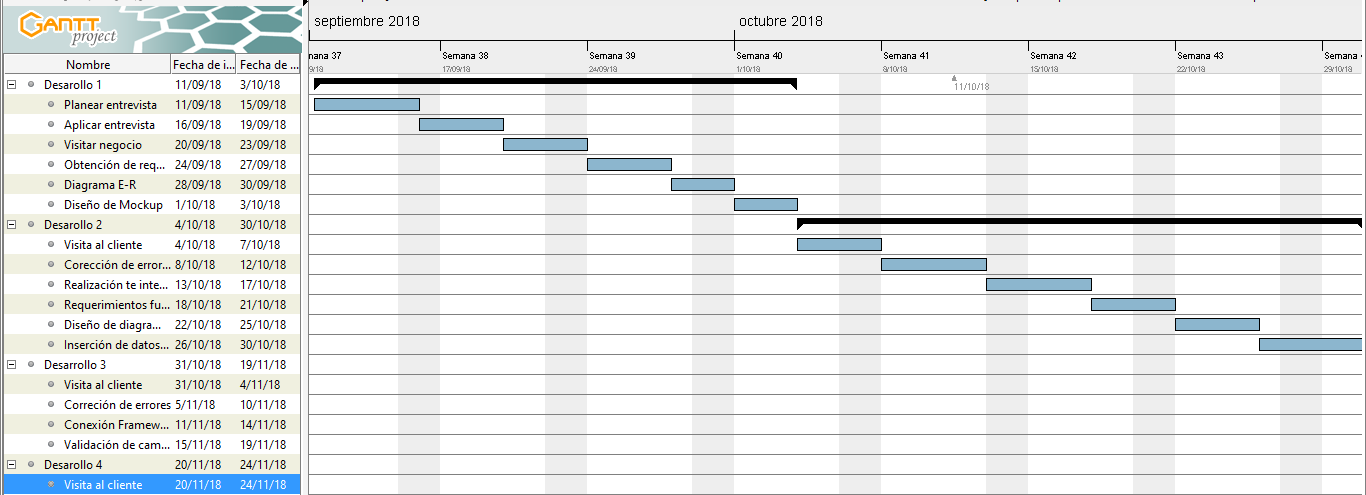
\includegraphics[width=15cm]{./imagenes/tablas/Diagrama_Gantt.png}
\end{center}

\end{figure}


El desarrollo de todo el proyecto tendrá una duración de 4 meses debido al ciclo de vida de la metodología elegida con anterioridad en la que se incluyen 5 visitas con el cliente, 3 retroalimentaciones y alrededor de 12 actividades descritas en la figura anterior.